\documentclass[12pt,letterpaper]{article}
\usepackage[utf8]{inputenc}
\usepackage[spanish]{babel}
\usepackage{graphicx}
\usepackage[left=2cm,right=2cm,top=2cm,bottom=2cm]{geometry}
\usepackage{graphicx} % figuras
% \usepackage{subfigure} % subfiguras
\usepackage{float} % para usar [H]
\usepackage{amsmath}
%\usepackage{txfonts}
\usepackage{stackrel} 
\usepackage{multirow}
\usepackage{enumerate} % enumerados
\renewcommand{\labelitemi}{$-$}
\renewcommand{\labelitemii}{$\cdot$}
% \author{}
% \title{Caratula}
\begin{document}

% Fancy Header and Footer
% \usepackage{fancyhdr}
% \pagestyle{fancy}
% \cfoot{}
% \rfoot{\thepage}
%

% \usepackage[hidelinks]{hyperref} % CREA HYPERVINCULOS EN INDICE

% \author{}
\title{Caratula}

\begin{titlepage}
\begin{center}
\large{UNIVERSIDAD PRIVADA DE TACNA}\\
\vspace*{-0.025in}
\begin{figure}[htb]
\begin{center}

\includegraphics[width=8cm]{./Imagenes/logo}
\end{center}
\end{figure}
\vspace*{0.15in}
INGENIERIA DE SISTEMAS  \\

\vspace*{0.5in}
\begin{large}
TITULO:\\
\end{large}

\vspace*{0.1in}
\begin{Large}
\textbf{ GITHUB} \\
\end{Large}

\vspace*{0.3in}
\begin{Large}
\textbf{CURSO:} \\
\end{Large}

\vspace*{0.1in}
\begin{large}
BASE DE DATOS II\\
\end{large}

\vspace*{0.3in}
\begin{Large}
\textbf{DOCENTE(ING):} \\
\end{Large}

\vspace*{0.1in}
\begin{large}
 Patrick Cuadros Quiroga\\
\end{large}

\vspace*{0.2in}
\vspace*{0.1in}
\begin{large}
Alumna: \\
\begin{flushleft}
Nelia Escalante Maron	           \hfill	(2014049551) \\
\end{flushleft}
\end{large}

\vspace*{0.3in}
\begin{Large}
\textbf{TACNA-PERU} \\
\end{Large}

\vspace*{0.1in}
\begin{large}
2018\\
\end{large}

\end{center}

\end{titlepage}

\vspace*{0.8in}
\begin{Large}
\part{Objetivo}
\begin{itemize}
\item Objetivo General
\item Saber y conocer sobre github 
\item Mas repositorios \\
\end{itemize}
\end{Large}

\vspace*{0.8in}
\part{Desarrollo del Trabajo}

\section{¿Qué es y para qué sirve GitHub?}
GitHub es una herramienta desconocida por muchos desarrolladores principiantes y que sin duda es de lo mejor que he podido aprender en mi tiempo que llevo programado, y se trata ni más ni menos que de los controladores de versiones, más concretamente Git y un servicio público llamado GitHub. Es importante revisar las herramientas para evitar dolores de cabeza y sobre todo nos permitirá mantener el código de una forma ordenada, por usuarios y sobretodo tener versiones por si alguna vez todo va mal y el proyecto poder salvarlo. 

Es importante saber que GitHub, es un servicio para mantener tu código a salvo del peligro, como sabemos las copias de seguridad de nuestros datos son importantes, tanto si son fotografías, ficheros o código de programación. 
Las alternativas siempre son las mismas: la nube usando Dropbox o Drive, en local usando discos duros aparte de los que empleamos para nuestro uso diario, pero en el caso del código tenemos una alternativa mucho mejor: los repositorios Git. Esta clase de repositorio son una copia local del código generado con una característica muy importante, y es que podemos hacer varias versiones para poder recular si nos hemos equivocado y nuestra aplicación ya no funciona, o para trabajar en funcionalidades nuevas sin necesidad de modificar la versión funcional y así no romper el proyecto. Esta es la premisa más básica de los repositorios de código, pero seguimos sin solucionar el tema de que se mantiene en local. Si nuestra máquina se estropea y deja de funcionar, corrompiendo el disco duro, no podemos recuperar todo el trabajo realizado. Es por ello que nacen servicios como GitHub, BitBucked u otros similares que pretenden llenar ese vacío.
Los usuarios de GitHub pueden utilizar Git o Subversion como VCS (Version Control System) para gestionar, revisar y preparar sus proyectos de software.

En el caso de los sistemas de gestión de versiones centralizados como CVS o SVN, el código fuente y otros archivos se almacenan en un repositorio o en un archivo de proyectos, desde donde pueden cargarse en otros ordenadores. Una vez terminada la edición, los archivos modificados pueden volver a introducirse en el repositorio, en cuyo caso la modificación también queda registrada.


\vspace*{-0.025in}
\begin{figure}[htb]
\begin{center}

\includegraphics[width=10cm]{./Imagenes/GithubN}
\end{center}
\end{figure}

\section{Ventajas e inconvenientes de usar GitHub}
\begin{itemize}
\item Una ventaja importante de GitHub es que el servicio pone a disposición de todos los usuarios repositorios de código públicos y libres sin límites. Sin embargo, el mantenimiento de repositorios privados está sujeto al pago de una suscripción mensual. GitHub también ofrece la posibilidad de crear “organizaciones” que hacen las veces de cuentas regulares a menos que tengas como mínimo una cuenta de usuario de tu propiedad.
\item A pesar de todo, en algunos casos puede haber ciertas limitaciones en lo relativo a la facilidad de uso y eficiencia de GitHub. En ocasiones surgen complicaciones entre el programa cliente y la compañía cuando, por ejemplo, un servidor privado opera como host para el código creado. Otra de las razones que motivan la elección de alternativas a GitHub es el empleo de un VCS diferente no soportado por GitHub. Hoy en día existen diversas alternativas a GitHub, pero en el presente artículo te hablamos de cinco de ellas.
\end{itemize}

\vspace*{-0.025in}
\begin{figure}[htb]
\begin{center}

\includegraphics[width=8cm]{./Imagenes/ventajas-uso-git}
\end{center}
\end{figure}

\part{ Mas alternativas }

\section{GitLab}
GitLab ofrece numerosas y útiles características en su DVCS, como, por ejemplo, un proyecto wiki integrado y una página web de proyecto. Las continuas capacidades de integración de GitLab automatizan el análisis y la entrega del código, lo que permite ahorrar tiempo en la fase de prueba. Con un visor de código, pull requests y un práctico método para solucionar conflictos, GitLab permite acceder a todos los aspectos importantes de tu proyecto. La aplicación está escrita en Ruby.

\vspace*{-0.025in}
\begin{figure}[htb]
\begin{center}
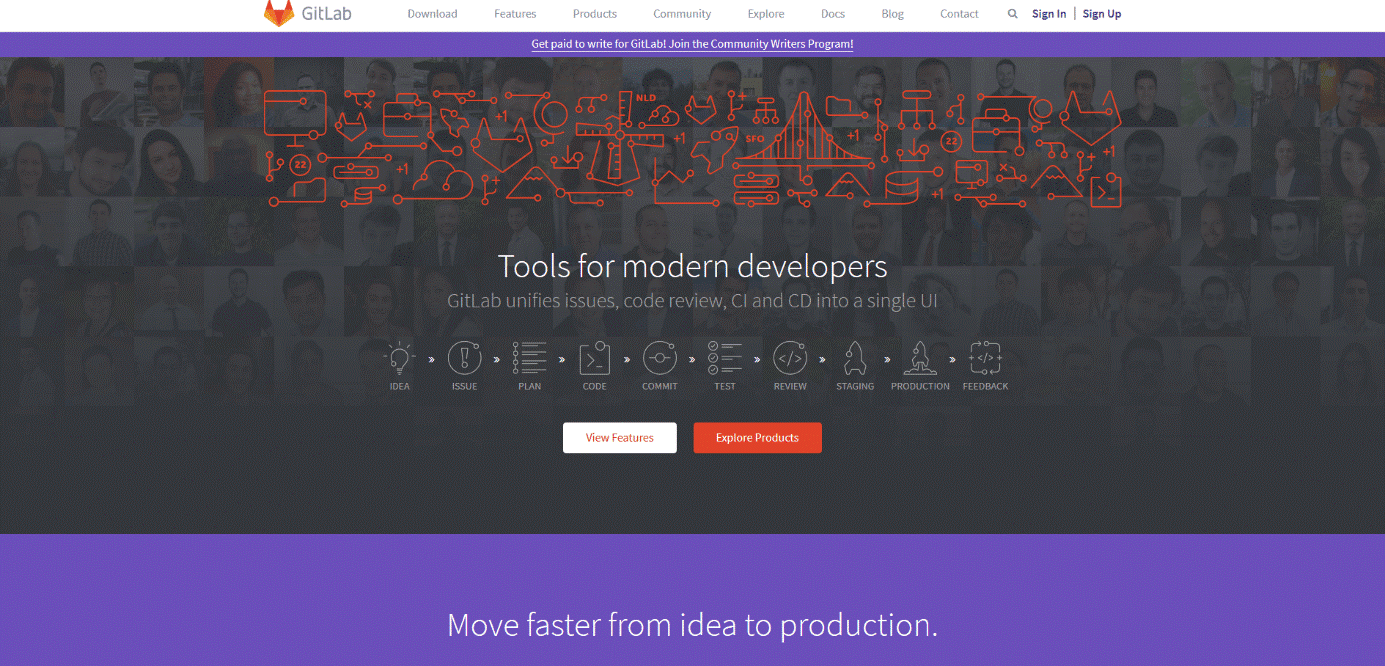
\includegraphics[width=16cm]{./Imagenes/gitlabN}
\end{center}
\end{figure}

\section{SourceForge}
A decir verdad, SourceForge ya estaba presente en el mercado antes de GitHub y de muchas otras alternativas open source y hubo una época en la que estaba considerada como la primera opción de código abierto. En 2015, la empresa tuvo algunos problemas con el malware, pero desde enero de 2016 va por el buen camino. Actualmente, SourceForge ofrece la autenticación multifactor, lo que armoniza con una orientación generalmente segura. Entre las características adicionales que pone a disposición de los usuarios se encuentran el sistema de seguimiento de incidentes y una lista de código incorporada.

\vspace*{-0.025in}
\begin{figure}[htb]
\begin{center}
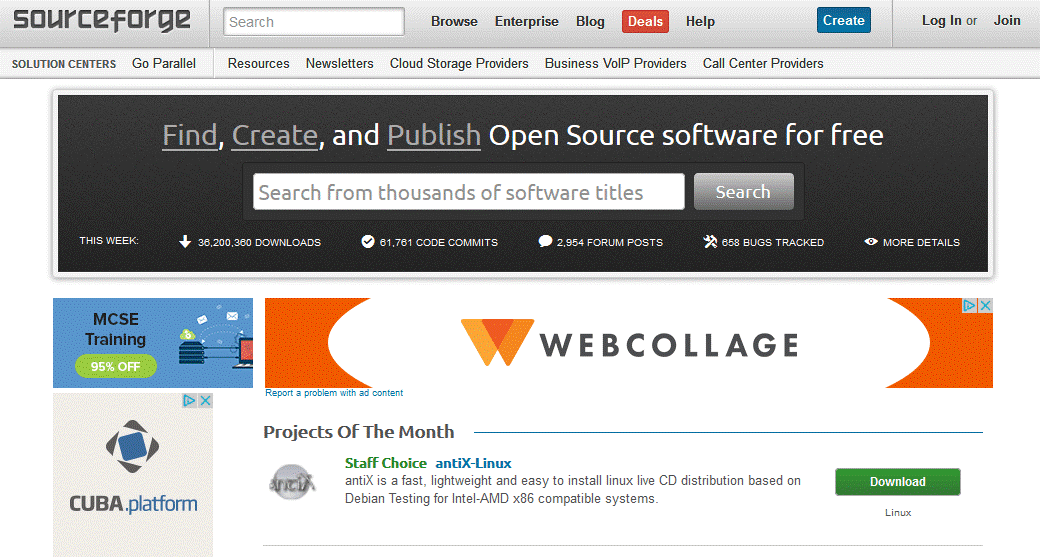
\includegraphics[width=16cm]{./Imagenes/2}
\end{center}
\end{figure}

\section{Cloud Source Repositories}
Tras el fracaso de Google Code, Cloud Source Repositories se encarga de la gestión de Google Cloud Platform. Con Cloud Source Repositories, que se encuentra en la versión beta, se pueden vincular otros repositorios vía GitHub o Bitbucket en función de las necesidades. En este caso, también es posible hacer uso de los repositorios propios de Google, los cuales se pueden guardar a través de la infraestructura de Google, lo que significa que tanto tu código como tus aplicaciones van de la mano.  La ventaja más importante de Cloud Source Repositories es que permite buscar código directamente a través del navegador. Asimismo, también tienes la posibilidad de detectar bugs con Cloud Diagnostics mientras el código se ejecuta en un segundo plano.

\vspace*{-0.025in}
\begin{figure}[htb]
\begin{center}
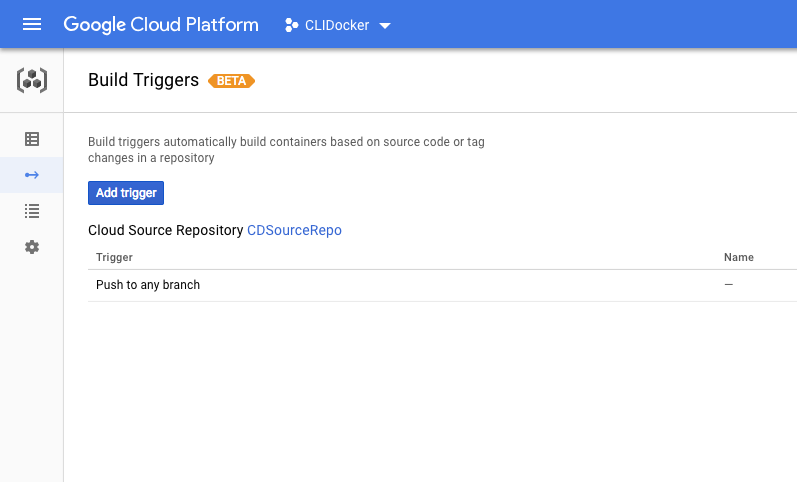
\includegraphics[width=10cm]{./Imagenes/6}
\end{center}
\end{figure}

\section{GitKraken}
GitKraken otorga un gran valor al ahorro de tiempo, algo que favorece a los usuarios a la hora de probar el código. Al sistema se le conoce, principalmente, por tener una interfaz muy vistosa, por centrarse en la velocidad y por el fácil manejo de Git. Con un práctico botón para deshacer operaciones se pueden revisar errores al momento, lo que hace más fácil el flujo de trabajo. La versión gratuita es apta para empresas con menos de 20 trabajadores o para organizaciones sin ánimo de lucro. La versión Pro, por su parte, ofrece características de gran utilidad, como por ejemplo el soporte de perfiles que permite separar proyectos con comodidad.

\vspace*{-0.025in}
\begin{figure}[htb]
\begin{center}

\includegraphics[width=16cm]{./Imagenes/4}
\end{center}
\end{figure}

\section{Mercurial}
Mercurial. El SCV distribuido Mercurial permite copiar un repositorio, conteniendo toda la historia del desarrollo del proyecto, esta copia del repositorio local funciona en forma independiente y autónoma sin requerir acceso a la red o a un servidor. La copia incluirá todos los archivos del proyecto y su historial. El repositorio local identifica la ubicación del repositorio origen, pero Mercurial no se comunicará con ese repositorio, a menos que el desarrollador lo realice. Mercurial tiene una interfaz de web de gran alcance que ofrece las siguientes funciones: navegación sobre la estructura de repositorios, visualización del historial de cambios, despliegue del contenido de directorios y archivos, utilización de Atom y RSS para estar al tanto de los cambios en el repositorio, soporta usuarios remotos para copiar, modificar y actualizar repositorios. El sistema Mercurial permite, mediante una extensión convert, importar proyectos de aplicaciones como Subversion, CVS, Git, Darcs, convertiendo toda la historia del proyecto en uno nuevo en el repositorio Mercurial. Adicionalmente, la extensión convert permite exportar los cambios a Subversion, posibilitando el llevar a cabo en paralelo el desarrollo de un proyecto.

\vspace*{-0.025in}
\begin{figure}[htb]
\begin{center}

\includegraphics[width=10cm]{./Imagenes/Mercurial}
\end{center}
\end{figure}

\part{ }
\section{Conclusiones}
Los sistemas de control de versiones ofrecen un soporte muy importante en el proceso de desarrollo de software, coadyuvando en la gestión del control de versiones de los archivos de código fuente e impulsando el trabajo colaborativo al permitir que múltiples desarrolladores trabajen paralelamente en un mismo proyecto en forma autónoma e independiente. Adicionalmente, los sistemas de control de versiones proporcionan los mecanismos para que cualquier versión de un proyecto pueda ser recuperada para visualizarse o modificarse, desplegando las diferencias entre las versiones existentes. Por otro lado, el desarrollo distribuido es soportado a través de redes de datos con diferentes mecanismos de autentificación. En el presente trabajo de investigación se presentó un análisis de los sistemas de control de versiones, tanto “open-source” como propietarios, describiendo las principales funciones que ofrecen al momento de realizar una implementación y/o aplicación en el desarrollo de software. Además, se define el proceso de creación y actualización de repositorios, tanto en el enfoque centralizado como distribuido, detallándose el proceso de actualización de archivos de código fuente de acuerdo a cada una de las herramientas revisadas. Cabe destacar que la presente investigación servirá como base teórica para el desarrollo de una herramienta para el control de versiones basado en servicios web que el grupo de investigación tiene planeado desarrollar en un futuro y cuyo fundamento se contempla dentro de las líneas de investigación y de los proyectos vigentes del cuerpo académico.

\part{ Webgrafia}
\begin{itemize}
\item Alternativas a GitHub 
https://www.1and1.es/digitalguide/paginas-web/desarrollo-web/alternativas-a-github-las-5-mejores-aplicaciones/

\item -	Sistema de versiones  
file:///C:/Users/Nelia/Downloads/Dialnet-RevisionDeLosSistemasDeControlDeVersionesUtilizado-4694154.pdf 

\item -	5 mejores alternativas 
 https://computerhoy.com/reportajes/tecnologia/5-mejores-alternativas-github-2018-275973

\item -	Sistema control de versiones 
http://rodin.uca.es/xmlui/bitstream/handle/10498/9785/trabajoSCV.pdf 

\item -	club de tecnología 
http://www.clubdetecnologia.net/blog/2017/github-vs-gitlab-vs-bitbucket-que-repositorio-elegir/ 

\end{itemize}

\end{document}
